% !TeX spellcheck = en_US
% !TeX encoding = UTF-8
\documentclass[11.5pt,aspectratio=1610,xcolor={usenames,dvipsnames,table}]{beamer}
\mode<presentation>
\usepackage[T1]{fontenc}
\usepackage[utf8]{inputenc}
\usepackage[english]{babel}
\usepackage{lmodern}
\usepackage[babel,style=english,english=american]{csquotes}
\usepackage{mathabx}
\usepackage{latexsym}
\usepackage{graphicx}
\usepackage{multicol}
\usepackage{multirow}
\usepackage[gen]{eurosym}
\usepackage{pgfpages}
\usepackage{xspace}
\usepackage{appendixnumberbeamer}
\usepackage[binary-units]{siunitx}
\usepackage{tabu}
\usepackage{graphicx}
\usepackage{pgfgantt}
%\usepackage{biblatex}

%\setcounter{tocdepth}{2}

%\usetheme[numbering=counter,progressbar=frametitle]{metropolis}
%\usetheme[numbering=none]{metropolis}
\usetheme[sectionpage=none,subsectionpage=none,numbering=counter,progressbar=none]{metropolis}
\usepackage{bibentry}
\usepackage[justification=centering]{caption}
%\usepackage[square,numbers]{natbib}
\definecolor{brsu_blue}{HTML}{0BA1E2}
\usepackage{url}
\usepackage[font=small]{caption} 
\usepackage[font=footnotesize]{subcaption}
\setbeamercolor{title separator}{fg=brsu_blue}
\setbeamercolor{progress bar}{fg=brsu_blue}
\setbeamercolor{normal text}{fg=black,bg=white}
\setbeamercolor{frametitle}{bg=brsu_blue,fg=white}
\usepackage{gensymb}

\title{Read Digits from Natural Images using Convolutional Neural Network}

%\titlegraphic{\includegraphics[width=5cm]{gfx/logo}}

\author{Ramesh Kumar \\ Roberto Cai Wu}

\date{\today}

\setbeamertemplate{caption}{\raggedright\insertcaption\par}



\setbeamerfont{footnote}{size=\tiny}






\begin{document}

\begin{frame}
\titlepage
\end{frame}


\section{Motivation}
\begin{frame}
	\frametitle{ Motivation}
	
	\begin{figure}[!h]
		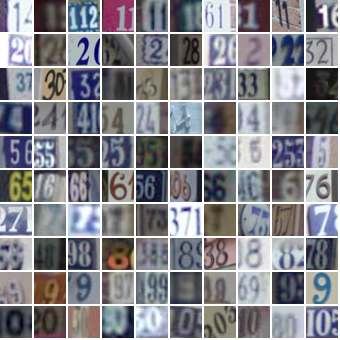
\includegraphics[height = 6cm]{images/dataset.png}
		\caption{Digit Recognition \cite{SVHN}}
	\end{figure}
	
	%\begin{itemize}
	%	\item This is a optical character recognition (OCR) problem
	%	\item Digit recognition is used in various applications such as postal mail
	%	sorting, bank check processing, form data entry, etc
	%	\item Digit recognition is an important component of modern-day map making \cite{Goodfellow2013}
		%\item It is a challenging problem due to:  \cite{Goodfellow2013}
	%\end{itemize}
\end{frame}

\section{Problem Description}
\begin{frame}
\frametitle{Problem Description}
\begin{itemize}
	\item Task is to read digits from natural images
	\item We use the MNIST dataset \cite{mnist}, which consists of hand-written digits
	\item Convolutional neural networks(CNN) for classification of digits
	\item Computer Vision techniques for detection of digits
\end{itemize}

\end{frame}


\section{Challenges}
\begin{frame}
\frametitle{Challenges(1)}


\begin{figure}[!h]
	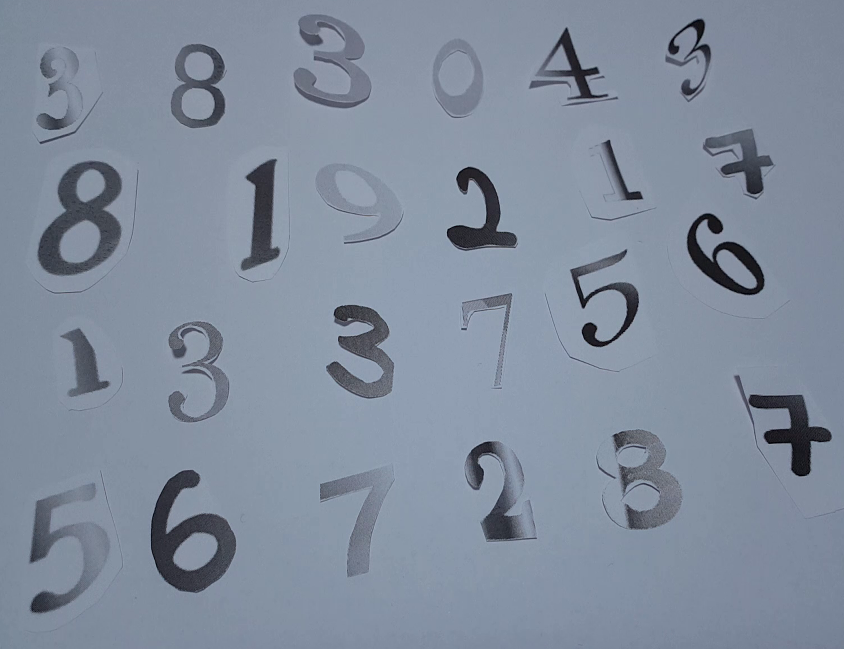
\includegraphics[scale=0.3 ]{images/chalorig.png}
	\caption{Image contains digits with shadows and different fonts}
\end{figure}

\end{frame}




\begin{frame}
\frametitle{Challenges(2)}


\begin{figure}[!h]
	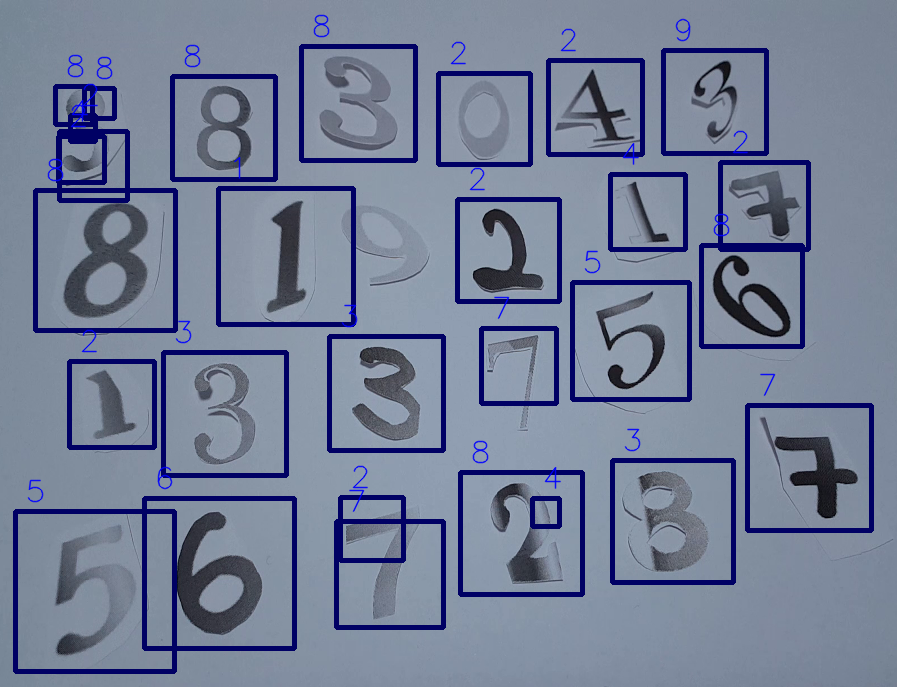
\includegraphics[scale=0.3 ]{images/chalbbox.png}
	\caption{Image with digits and bounding boxes}
\end{figure}

\end{frame}

\section{Assumptions}
\begin{frame}
\frametitle{Assumptions}
\begin{itemize}
	\item Images contain only digits.
	\item Background is a solid color and does not change
	\item Numbers should be distanced enough so that bounding boxes do not overlap.
	\item Digits are visible to camera, orientations may be varied till 45$^{\circ}$ or 60$^{\circ}$ 
	%\item We may be able to detect digits with blurred images as data set contains blurred images

\end{itemize}
\end{frame}

\section{Setup}

\begin{frame}
\frametitle{Setup}
	\begin{itemize}
		\item Camera; we use mobile camera
		\item Solid background with suitable font color 
		\item Suitable lighting conditions
	\end{itemize}



\end{frame}


\section{Methodology}
\begin{frame}

\frametitle{Methodology}
%\myheading{\textbf{Block Diagram}}

\begin{itemize}
	\item Load and Interpret DataSet
	\item Pre-processing(dataset as well as live camera)
	\item Convolutional Neural Network
	\item Post-processing(during camera only)
	\item Testing and evaluation
\end{itemize}
\begin{figure}[!h]
	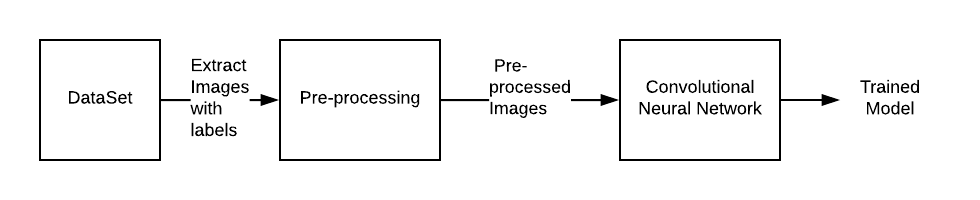
\includegraphics[width=\textwidth ]{images/methodology_1.png}
	\caption{Block Diagram of System using Dataset}
\end{figure}

\end{frame}

\begin{frame}

\frametitle{Methodology contd..}

\begin{figure}[!h]
	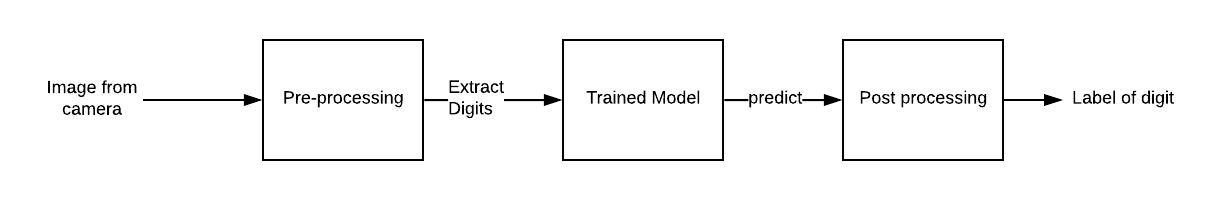
\includegraphics[width=\textwidth ]{images/methodology_2.png}
	\caption{Block Diagram of System using Camera}
\end{figure}


\end{frame}


%% 
\begin{frame}

\frametitle{MNIST Dataset \cite{mnist}  }

\begin{itemize}
	\item 10 classes, 1 for each digit
	\item Digit 1 has label 1,9 has label 9, and 0 has label 10
	\item 60,000 digits for training, 10,000 digits for testing
	\item Digits are arranged in different positions with solid background
\end{itemize}

\end{frame}


\begin{frame}

\section{Dataset}
\frametitle{DataSet}

\begin{figure}[!h]
	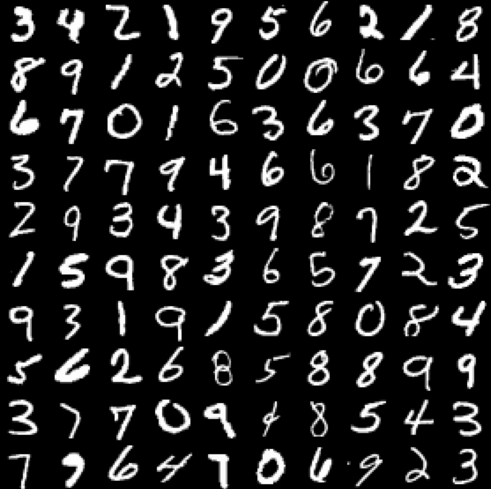
\includegraphics[height = 6cm]{images/mnist-digits-small.png}
	\caption{Example images from MNIST dataset \cite{mnist}}
\end{figure}

\end{frame}


\section{Pre-processing from camera}
\begin{frame}
\frametitle{Pre-processing from camera}

\begin{itemize}
	\item Resize image to 640x480 pixels
	\item Convert to gray scale
	\item Apply Gaussian filter
	\item Use a binary thresholding
	\item Find contours
	\item Draw bounding box around contours
\end{itemize}
\end{frame}

\begin{frame}
\frametitle{Pre-processing from camera(2)}

\begin{figure}[!h]
	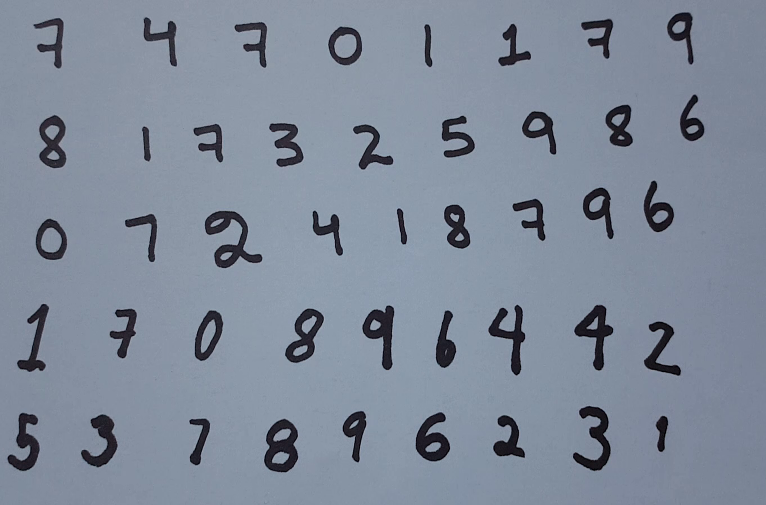
\includegraphics[height = 6cm]{images/orig.png}
	\caption{Image taken from live camera }
\end{figure}

\end{frame}

\begin{frame}
\frametitle{Pre-processing from camera (3)}

\begin{figure}[H]
	

	\centering
	\begin{subfigure}{0.4\textwidth}
	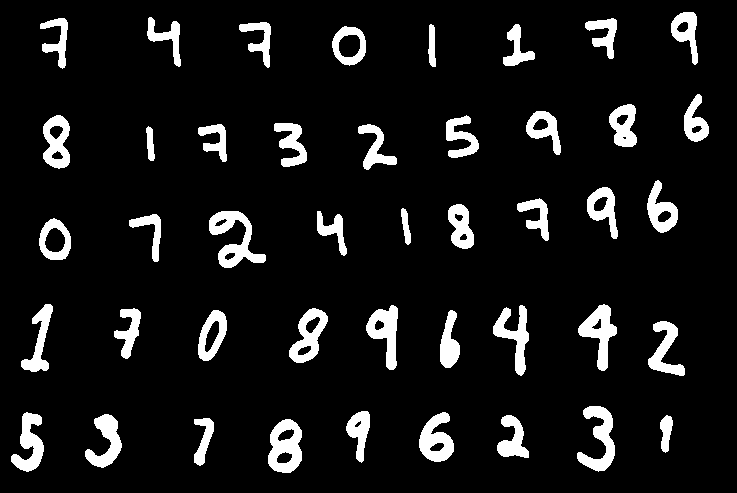
\includegraphics[width=0.8 \textwidth]{images/thresh.png}
	\caption{Binary threshold image}
	\end{subfigure}
	
	\begin{subfigure}{0.4\textwidth}
		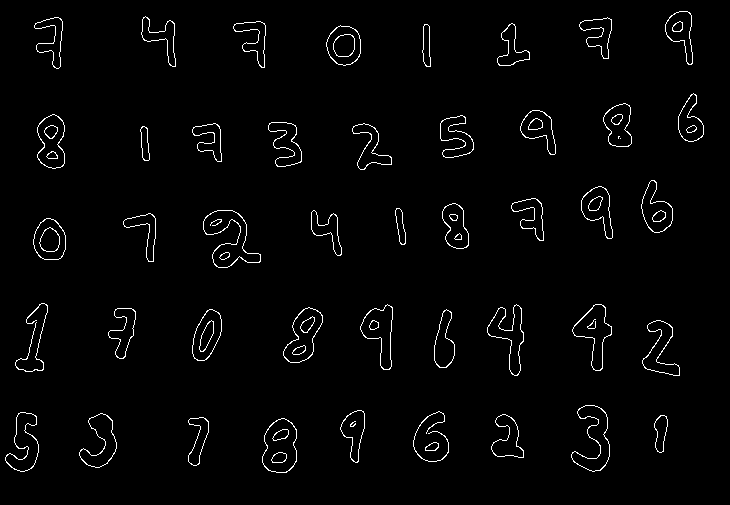
\includegraphics[width=0.8 \textwidth]{images/edge.png}
		\caption{Canny edge detector}
	\end{subfigure}
	
\end{figure}

\end{frame}








\begin{frame}
\frametitle{Pre-processing from camera (4)}
	
\begin{figure}[!h]
	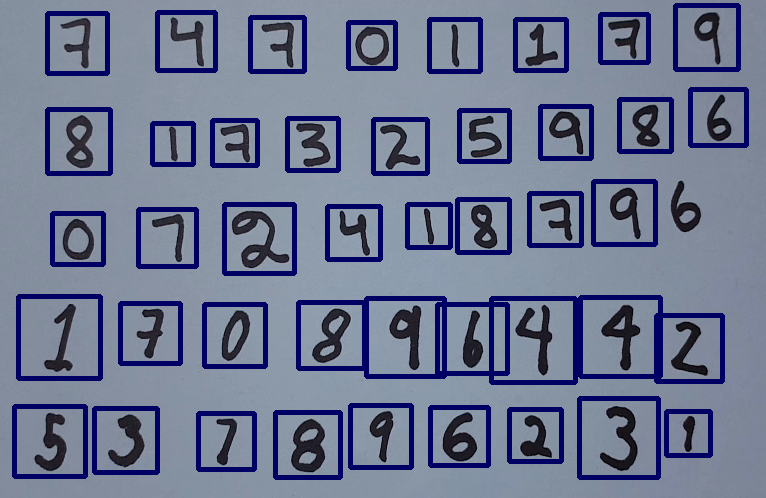
\includegraphics[height = 6cm]{images/bbox.png}
	\caption{Bounding boxes drawn over original image}
\end{figure}
\end{frame}



\section{CNN}

\begin{frame}

\frametitle{Convolutional Neural Network(CNN)}

\begin{itemize}
	\item State-of-the-art shows CNN performs better as compare to other approaches\cite{cnn}
	\item Extracts features from the images and classify them
	\item Three type of layers
		\begin{itemize}
			\item Convolutional: Extract low-level and high-level features
			\item Pooling: Reduce amount of parameters and computations
			\item Fully Connected: Neurons are fully connected
		\end{itemize}	
	\begin{figure}[!h]
		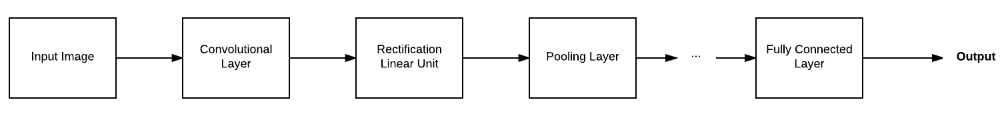
\includegraphics[width=\textwidth]{images/cnn.png}
		\caption{Basic Architecture of CNN }
		
	\end{figure}

\end{itemize}
\end{frame}

\begin{frame}

\frametitle{Our CNN Model}


\begin{figure}[!h]
	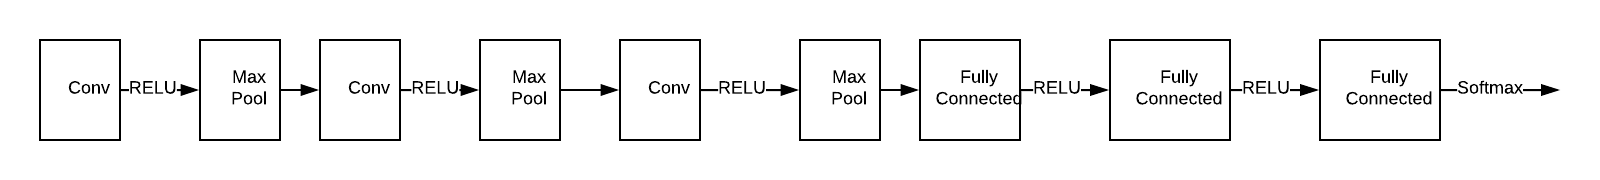
\includegraphics[width=\textwidth]{images/cnn_model.png}
	\caption{Model used to train MNIST dataset }
	
\end{figure}


\end{frame}
%% post processing

%\begin{frame}
%\frametitle{Post-processing}
%
%\begin{itemize}
%	\item After classification, we use adaptive 
%\end{itemize}
%
%\end{frame}

\begin{frame}
\frametitle{Testing \& Evaluation(1)}

\begin{itemize}
	\item Print/write numbers on a sheet of paper (different size, font, color,  and orientation)
	\item Test the images of digits from live camera under different conditions (light and perspective)
	\item Use test set to compute accuracy of model, gives us 99.13\%
\end{itemize}
\end{frame}





\begin{frame}
\frametitle{Testing \& Evaluation(2)}



\begin{figure}[H]
	
	
	
	\begin{subfigure}{0.7\textwidth}
		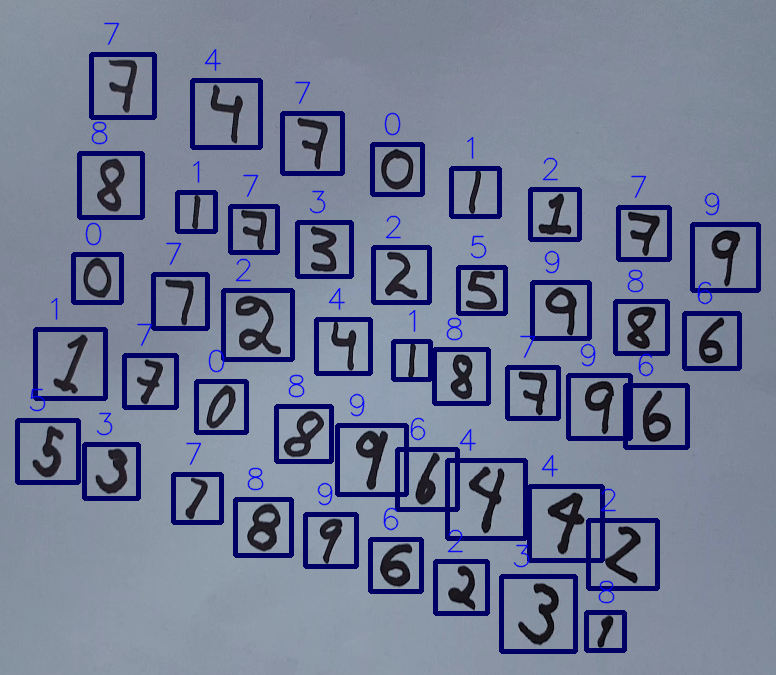
\includegraphics[width=0.5 \textwidth]{images/bbox_p3.png}
		\caption{Detection of digits with different orientations}
	\end{subfigure}
	
	\begin{subfigure}{0.7\textwidth}
		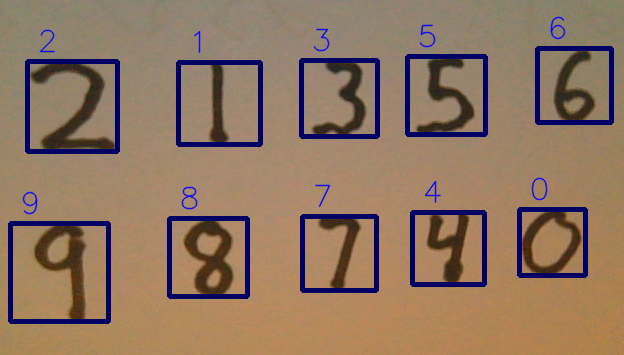
\includegraphics[width=0.5 \textwidth]{images/bbox_p11.png}
		\caption{Detection of digits}
	\end{subfigure}
	
\end{figure}



\end{frame}

\bibliographystyle{unsrt}
\nocite*
\bibliography{presentation.bib}

%\begin{thebibliography}{9}
%\bibitem{MdArfat}
%Md Arafat Sultan, Cristobal Salazar and Tamara Sumner, "Fast and Easy Short Answer Grading with High Accuracy", Conference of the North American Chapter of the Association for Computational Linguistics: Human Language Technologies, San Diego California, USA, June 12-17, 2016
%\bibitem{Sultan_wordAligner}"Md Arafat Sultan
%	, Steven Bethard and Tamara Sumner", "Back to Basics for Monolingual Alignment: Exploiting Word Similarity and
%	Contextual Evidence",  TACL, 2014
%
%\bibitem{Nlp}
%Speech and Language Processing by Daniel Jurafsky and James H. Martin
%\bibitem{lemmaAndStemma}
% https://queryunderstanding.com/stemming-and-lemmatization-6c086742fe45
%
%\bibitem{n-gram}
% http://www.dictionary.com/browse/n-gram
%
%
%\end{thebibliography}


\end{document}
